\documentclass[portrait, color=UCLburgundy, margin=1cm]{uclposter}

\newcommand{\boldf}{\bm{f}}
\newcommand{\boldmu}{\bm{\mu}}
\newcommand{\boldalpha}{\bm{\alpha}}
\newcommand{\boldr}{\bm{r}}
\newcommand{\boldt}{\bm{t}}
\newcommand{\boldg}{\bm{g}}
\newcommand{\boldtheta}{\bm{\theta}}

% Warping operators
\newcommand{\MPWarp}{\tilde{\mathcal{W}}}
\newcommand{\Warp}{\mathcal{W}}

% Others
\newcommand{\etal}{\textit{et al.}~}
\newcommand{\ie}{i.e., }
\newcommand{\eg}{e.g., }

\usepackage{bm}
\usepackage{algorithm}
\usepackage{algorithmic}
\usepackage{caption}
\usepackage{blindtext}
\usepackage{siunitx}

\usepackage[acronym, nomain]{glossaries}

% Define "long-s" key: 
\glsaddkey* {longs}% key 
{\glsentrylong{\glslabel}s}% default value 
{\glsentrylongs}% command analogous to \glsentrytext 
{\Glsentrylongs}% command analogous to \Glsentrytext 
{\glslongs}% command analogous to \glstext 
{\Glslongs}% command analogous to \Glstext 
{\GLSlongs}% command analogous to \GLStext

%% Define "short-s" key: 
\glsaddkey* {shorts}% key 
{\glsentryshort{\glslabel}s}% default value 
{\glsentryshorts}% command analogous to \glsentrytext 
{\Glsentryshorts}% command analogous to \Glsentrytext 
{\glsshorts}% command analogous to \glstext 
{\Glsshorts}% command analogous to \Glstext 
{\GLSshorts}% command analogous to \GLStext

\DeclareRobustCommand{\glss}[1]
{%
  \ifglsused{#1}{\glsshorts{#1}}{\glslongs{#1} (\glsshorts{#1})\glsunset{#1}}%
}

\DeclareRobustCommand{\Glss}[1]
{%
  \ifglsused{#1}{\Glsshorts{#1}}{\Glslongs{#1} (\glsshorts{#1})\glsunset{#1}}%
}

\newacronym{18F-FDG}{18F-FDG}{Fluorine-$18$ Fludeoxyglucose}
\newacronym{1D}{1D}{$1$-Dimensional}
\newacronym{2D}{2D}{$2$-Dimensional}
\newacronym{3D}{3D}{$3$-Dimensional}
\newacronym[longs={$3$-Dimensional Point Clouds}, shorts={3DPCs}]{3DPC}{3DPC}{$3$-Dimensional Point Cloud}
\newacronym{4D}{4D}{$4$-Dimensional}
% \newacronym{4DCT}{4DCT}{$4$-Dimensional Computed Tomography}
\newacronym{4DCT}{4DCT}{$4$D Computed Tomography}
\newacronym{ACF}{ACF}{Attenuation Correction Factors}
\newacronym{AC}{AC}{Attenuation Corrected}
\newacronym{AD}{AD}{Affine Deformation}
\newacronym{AP}{AP}{Anterior Posterior}
\newacronym{ATP}{ATP}{Adenosine Triphosphate}
% \newacronym{AV-CCT}{AV-CCT}{Averaged CINE-Computed Tomography}
\newacronym{AV-CCT}{AV-CCT}{Averaged CINE-CT}
\newacronym{BE}{BE}{Bending Energy}
\newacronym{BFGS}{BFGS}{Broyden Fletcher Goldfarb Shanno}
\newacronym{CC}{CC}{Correlation Coefficient}
% \newacronym{CCT}{CCT}{CINE-Computed Tomography}
\newacronym{CCT}{CCT}{CINE-CT}
\newacronym{CG}{CG}{Conjugate Gradient}
\newacronym{COM}{COM}{Centre of Mass}
\newacronym[longs={Control Points}, shorts={CPs}]{CP}{CP}{Control Point}
\newacronym[longs={Control Point Grids}, shorts={CPGs}]{CPG}{CPG}{Control Point Grid}
\newacronym{CT}{CT}{Computed Tomography}
\newacronym{DDG}{DDG}{Data Driven Gating}
\newacronym{DD-PCA}{DD-PCA}{Data Driven Principal Component Analysis Surrogate Signal Extraction}
\newacronym{DD}{DD}{Data Driven}
\newacronym[longs={Deformation Vector Fields}, shorts={DVFs}]{DVF}{DVF}{Deformation Vector Field}
\newacronym{EANM}{EANM}{European Association of Nuclear Medicine}
\newacronym{EM}{EM}{Expectation Maximisation}
\newacronym{FDG}{FDG}{Fluorodeoxyglucose}
\newacronym{FFT}{FFT}{Fast Fourier Transform}
\newacronym[longs={Fields of View}, shorts={FOVs}]{FOV}{FOV}{Field Of View}
\newacronym{FWHM}{FWHM}{Full Width at Half Maximum}
\newacronym{GAN}{GAN}{Generative Adversarial Networks}
\newacronym{GD}{GD}{Gradient Descent}
\newacronym{GE}{GE}{General Electric}
\newacronym{GT}{GT}{Ground Truth}
\newacronym{HU}{HU}{Hounsfield Unit}
\newacronym[longs={Image Registrations}, shorts={IRs}]{IR}{IR}{Image Registration}
\newacronym{KBq/mL}{KBq/mL}{Kilo Becquerel per Millilitre}
\newacronym{KeV}{KeV}{Kilo Electron Volt}
\newacronym{KRG}{KRG}{Kinetic Respiratory Gating}
\newacronym{KV}{KV}{Kilo Volt}
\newacronym{L-BFGS-B}{L-BFGS-B}{Low memory Broyden Fletcher Goldfarb Shanno Bounded}
\newacronym{L-BFGS}{L-BFGS}{Low memory Broyden Fletcher Goldfarb Shanno}
\newacronym[longs={Light Emitting Diodes}, shorts={LEDs}]{LED}{LED}{Light Emitting Diode}
\newacronym{LE}{LE}{Linear Energy}
\newacronym[longs={Lines of Response}, shorts={LORs}]{LOR}{LOR}{Line of Response}
\newacronym{LM}{LM}{Lateral Medial}
\newacronym{LR}{LR}{Linear Regression}
\newacronym{MAE}{MAE}{Mean Absolute Error}
\newacronym{MAD}{MAD}{Median Absolute Difference}
\newacronym{MAPE}{MAPE}{Mean Absolute Percentage Error}
\newacronym{MBF}{MBF}{Myocardial Blood Flow}
\newacronym{MCIR}{MCIR}{Motion Compensated Image Reconstruction}
\newacronym[longs={Motion Compensated Images}, shorts={MCIs}]{MCI}{MCI}{Motion Compensated Image}
\newacronym{MC}{MC}{Motion Correction}
\newacronym{MIC}{MIC}{Medical Imaging Convention}
\newacronym{MI}{MI}{Mutual Information}
\newacronym{ML}{ML}{Maximum Likelihood}
\newacronym{MLAA}{MLAA}{Maximum Likelihood Reconstruction of Activity and Attenuation}
\newacronym{MLACF}{MLACF}{Maximum Likelihood Activity and Attenuation Correction Factors Estimation}
\newacronym{MLE}{MLE}{Maximum Likelihood Estimation}
\newacronym{MLEM}{MLEM}{Maximum Likelihood Expectation Maximisation}
\newacronym[longs={Motion Models}, shorts={MMs}]{MM}{MM}{Motion Model}
\newacronym{MPI}{MPI}{Myocardial Perfusion Imaging}
\newacronym{MR}{MR}{Magnetic Resonance}
\newacronym{MSc}{MSc}{Master of Science}
\newacronym{MSE}{MSE}{Mean Squared Error}
\newacronym[longs={Attenuation Maps}, shorts={Mu-Maps}]{Mu-Map}{Mu-Map}{Attenuation Map}
\newacronym{NAC}{NAC}{Non-Attenuation Corrected}
\newacronym{NMI}{NMI}{Normalised Mutual Information}
\newacronym{ND}{ND}{$n$-Dimensional}
\newacronym{NMC}{NMC}{Non-Motion Corrected}
\newacronym{NN}{NN}{Neural Network}
\newacronym{NRD}{NRD}{Non-Rigid Deformation}
\newacronym{NTOF}{NTOF}{Non-Time-of-Flight}
\newacronym{OSEM}{OSEM}{Ordered Subset Expectation Maximisation}
\newacronym[longs={Principal Components}, shorts={PCs}]{PC}{PC}{Principal Component}
\newacronym{PCA}{PCA}{Principal Component Analysis}
\newacronym{PCC}{PCC}{Pearson Correlation Coefficient}
\newacronym{PET}{PET}{Positron Emission Tomography}
\newacronym{PLL}{PLL}{Poisson Log Likelihood}
\newacronym{PSD}{PSD}{Power Spectral Density}
\newacronym{PSMA}{PSMA}{Prostate Specific Membrane Antigen}
\newacronym{RANSAC}{RANSAC}{Random Sample Consensus}
\newacronym{RCM}{RCM}{Respiratory Correspondence Model}
\newacronym{RD}{RD}{Rigid Deformation}
\newacronym{RDP}{RDP}{Relative Difference Prior}
\newacronym{RM}{RM}{Respiratory Motion}
\newacronym{RMC}{RMC}{Respiratory Motion Correction}
\newacronym{RMSE}{RMSE}{Root Mean Square Error}
\newacronym[longs={Regions of Interest}, shorts={ROIs}]{ROI}{ROI}{Region of Interest}
\newacronym{RPM}{RPM}{Real Time Position Management}
\newacronym{RTPM}{RTPM}{Real Time Position Management}
\newacronym{SAM}{SAM}{Spectral Analysis Method}
\newacronym{SGD}{SGD}{Stochastic Gradient Descent}
\newacronym{SI}{SI}{Superior Inferior}
\newacronym{SIRF}{SIRF}{Synergistic Image Reconstruction Framework}
\newacronym{SNR}{SNR}{Signal to Noise Ratio}
\newacronym[longs={Surrogate Signals}, shorts={SSs}]{SS}{SS}{Surrogate Signal}
\newacronym{SSD}{SSD}{Sum of Squared Differences}
\newacronym{SSIM}{SSIM}{Structural Similarity Index Measure}
\newacronym{STFT}{STFT}{Short-time Fourier transform}
\newacronym{STIR}{STIR}{Software for Tomographic Image Reconstruction}
\newacronym{SUV}{SUV}{Standard Uptake Value}
\newacronym{SVD}{SVD}{Singular Value Decomposition}
\newacronym{TOF}{TOF}{Time-of-Flight}
\newacronym{TPS}{TPS}{Thin Plate Spline}
\newacronym{XCAT}{XCAT}{$4$-Dimensional Extended Cardiac Torso}

% \glsunset{18F-FDG}
% \glsunset{1D}
% \glsunset{2D}
% \glsunset{3D}
% \glsunset{4D}
% \glsunset{4DCT}
% \glsunset{ATP}
% \glsunset{BFGS}
% \glsunset{CT}
% \glsunset{EANM}
% \glsunset{FDG}
% \glsunset{GE}
% \glsunset{L-BFGS-B}
% \glsunset{L-BFGS}
% \glsunset{LED}
% \glsunset{MIC}
% \glsunset{MLAA}
% \glsunset{MLEM}
% \glsunset{MR}
% \glsunset{MSc}
% \glsunset{Mu-Map}
% \glsunset{NTOF}
% \glsunset{OSEM}
% \glsunset{PCA}
% \glsunset{PET}
% \glsunset{RANSAC}
% \glsunset{RPM}
% \glsunset{RTPM}
% \glsunset{SIRF}
% \glsunset{STIR}
% \glsunset{SUV}
% \glsunset{TOF}
% \glsunset{XCAT}


\usepackage[style=ieee, maxbibnames=1, minbibnames=1, maxcitenames=1, mincitenames=1, backend=biber, defernumbers=false]{biblatex}
\addbibresource{./Biblio.bib}

\AtEveryBibitem{\clearfield{month}}
\AtEveryBibitem{\clearfield{day}}
\AtEveryBibitem{\clearfield{volume}}
\AtEveryBibitem{\clearfield{issue}}
\AtEveryBibitem{\clearfield{pages}}
\AtEveryBibitem{\clearfield{number}}
\AtEveryBibitem{\clearfield{title}}
\AtEveryBibitem{\clearfield{isbn}}
\AtEveryBibitem{\clearfield{keywords}}
\AtEveryBibitem{\clearfield{issn}}
\AtEveryBibitem{\clearfield{journal}}

\usepackage{fontspec}
\setmainfont[Ligatures=TeX]{LexendDeca-Regular.ttf}

\begin{document}
    \title{PET/CT Motion Correction Exploiting Motion Models Fit \newline~on Coarsely Gated Data Applied to Finely Gated Data}
    
    \author[12*]{Alexander~C.~Whitehead}
    \author[3]{Kuan-Hao~Su}
    \author[3]{Scott~D.~Wollenweber}
    \author[2]{\newline~Jamie~R.~McClelland}
    \author[12]{Kris~Thielemans}
    
    \affil[1]{INM, UCL}
    \affil[2]{CMIC, UCL}
    \affil[3]{GE Healthcare}
    \affil[*]{alexander.whitehead.18@ucl.ac.uk}
    
    \maketitle

    \begin{multicols}{3}
        \section*{Introduction}
            \begin{highlightbox}[UCLlightgreen]
                \begin{itemize}
                    \item \glss{MM} parameterise \glss{DVF} in terms of a \gls{SS}.
                    \item \glss{MM} impose a degree of temporal or gate-wise regularisation.
                    \item \glss{MM} can obtain \glss{DVF} for unseen data~\cite{McClelland2013}).
                    \item Previous work~\cite{Whitehead2021ComparisonMap} indicated that \glss{MM} and \gls{TOF} increase resolution.
                    \item This work incorporates \acrshort{MLACF}~\cite{Nuyts2012ML-reconstructionFactors}.
                    \item This work incorporates a diffeomorphic velocity field parameterised registration
                    \item This work fits the \gls{MM} on coarsely gated data and applies it to finely gated data.
                    \item This work uses more realistic simulation and count levels.
                    \item This work differentiates itself by using two \glss{SS}, and group-wise registration.
                \end{itemize}
            \end{highlightbox}
        
        \section*{Methods}
            \subsection*{\underline{\textbf{\acrshort{XCAT} Volume Generation}}}
                \begin{itemize}
                    \item \acrshort{XCAT} generated 480 volumes using a 240 second respiratory trace.
                    \item Activity concentrations from a static \gls{18F-FDG} patient scan.
                    \item \gls{FOV} including the base of the lungs with a 20 millimetre diameter lesion.
                \end{itemize}
            
            \subsection*{\underline{\textbf{\acrshort{PET} Acquisition Simulation}}}
                \begin{itemize}
                    \item Simulated using the geometry of a \gls{GE} Discovery 710.
                    \item Pseudo-randoms and scatter were added.
                    \item Noise was simulated, such that data matched an acquisition over 240 seconds. The count rate was selected to match that of research scans
                    \item A respiratory \gls{SS} was generated using \gls{PCA}~\cite{Thielemans2011}.
                    \item Gated into four respiratory bins using the \gls{SS} and its gradient, each bin was a quadrant centred on the maximum or minimum of the displacement or gradient.
                    \item \gls{SS} values were determined for the post-gated data by taking an average of the \gls{SS} values in each bin.
                \end{itemize}
            
            \subsection*{\underline{\textbf{\acrshort{MLACF} Image Reconstruction}}}
                \begin{itemize}
                    \item Reconstructed using \acrshort{MLACF} with seven full iterations and 24 subsets for the activity update, and 9 iterations for the attenuation update~\cite{Nuyts2012ML-reconstructionFactors}.
                    \item Initialised using one iteration of \acrshort{MLEM}, with breath hold \acrshort{CT} for \gls{AC}.
                    \item Normalised between iterations and epsilon added.
                    \item Quadratic prior included in reconstruction.
                \end{itemize}
            
            \subsection*{\underline{\textbf{Registration}}}
                \begin{itemize}
                    \item Pre-processing including; replication of end-slices, smoothing, and standardisation.
                    \item Group-wise registration with initial pair-wise step.
                    \item Between each iteration, resampled volume was registered to the \gls{Mu-Map} and \glss{DVF} composed together.
                    \item Diffeomorphic velocity field b-spline registration using \gls{NMI}.
                    \item \acrlong{CPG} spacing, \acrlong{BE} weight and number of iterations tuned using a grid search.
                \end{itemize}
            
            \subsection*{\underline{\textbf{\acrlong{MM} Estimation}}}
                \begin{itemize}
                    \item \gls{MM} fit as direct \acrlong{RCM} using weighted \gls{LR} between registration \glss{DVF} and two \glss{SS}
                    \item \gls{LR} weight set from total counts in gate
                    \item \gls{MM} fit between each iteration.
                \end{itemize}
            
            \subsection*{\underline{\textbf{Image Reconstruction with AC}}}
                \begin{itemize}
                    \item Re-gatedinto 30 respiratory bins using displacement gating, \gls{SS} and its gradient (10 amplitude and three gradient bins).
                    \item \glss{Mu-Map} determined using the inverse of the \glss{DVF} from the \gls{MM}.
                    \item Re-reconstructed with \gls{AC} using \gls{OSEM} with two full iterations and 24 subsets.
                    \item Volumes post-filtered with a Gaussian smoothing, (\gls{FWHM} of 6.4 millimetre in transverse plane and a normal Z-filter).
                \end{itemize}
            
            \subsection*{\underline{\textbf{Evaluation}}}
                \begin{itemize}
                    \item Data were also \gls{MC} in the same way, but using high noise high temporal/gate resolution, or noiseless data, for the \gls{MM} fitting.
                    \item Data also reconstructed without \gls{MC}, using either a sum of all \glss{Mu-Map} or the end inhalation \gls{Mu-Map}.
                    \item Volumes without \gls{MC} registered to the position of the \gls{Mu-Map}.
                    \item \glss{DVF} generated by each method were also applied to noiseless data for visual analysis.
                    \item Comparisons used included: A visual analysis, \acrshort{SSIM} to the ground truth~\cite{Wang2009MeanMeasures}, a profile over the lesion, \gls{SUV}\textsubscript{max} and \gls{SUV}\textsubscript{peak}.
                \end{itemize}
        
        \section*{Conclusion}
            \begin{highlightbox}[UCLlightgreen]
                \begin{itemize}
                    \item A low number of gates for \gls{MM} fitting has minimal impact at low noise
                    \item A low number of gates for \gls{MM} fitting improves \gls{MC} when there is a high level of noise in the gates
                    \item The execution time using a reduced number of gates is lower.
                    \item In the future, work will focus on evaluating the method on patient data.
                \end{itemize}
            \end{highlightbox}
        
        \AtNextBibliography{\tiny}
        \printbibliography
    \end{multicols}
    
    \begin{multicols}{2}
        \begin{figure}[H]
            \centering
            
            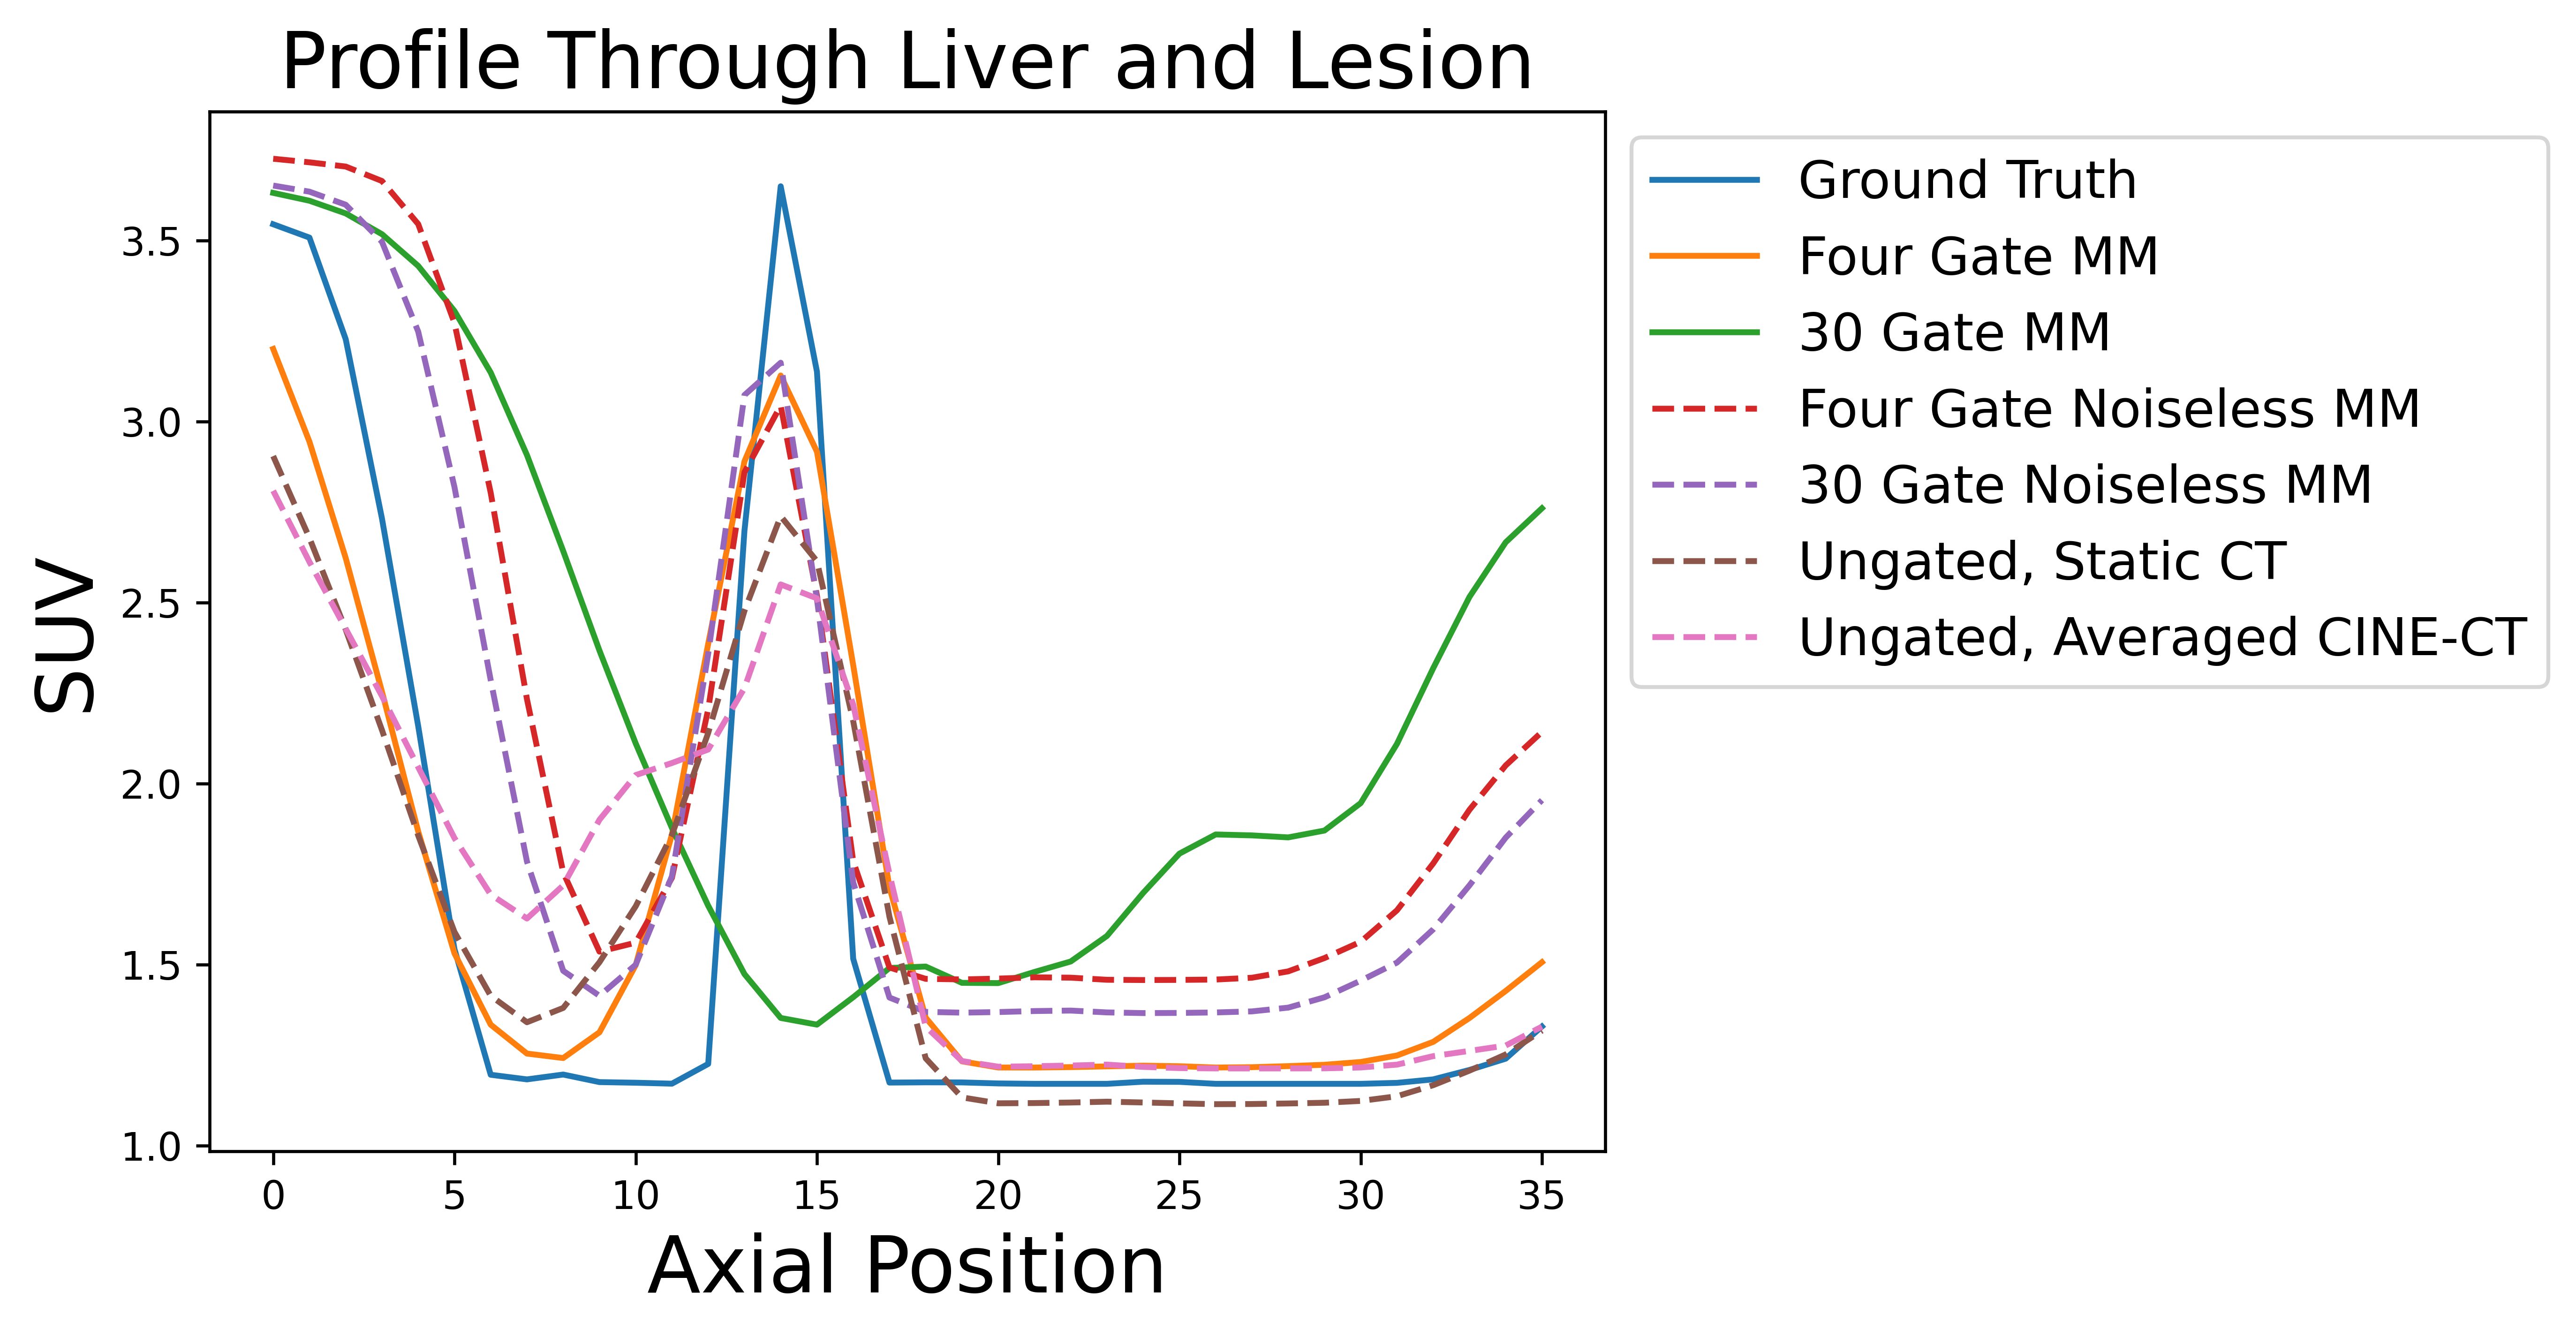
\includegraphics[width=1.0\linewidth]{profile.png}
            
            \begin{highlightbox}[UCLlightblue]
                \captionsetup{singlelinecheck=false, justification=centering}
                \caption{Profile across the lesion.}
            \end{highlightbox}
            
            \label{fig:profile}
        \end{figure}
        
        \begin{table}[H]
            \centering
            
            \begin{highlightbox}[UCLlightblue]
                \captionsetup{singlelinecheck=false, justification=centering}
                \caption{Comparison of \gls{SUV}\textsubscript{max} and \gls{SUV}\textsubscript{peak}.}
            \end{highlightbox}
            
            \vspace{1.0cm}
            
            \resizebox*{1.0\linewidth}{!}
            {
                \begin{tabular}{||c|cc||}
                    \hline
                    \textbf{\acrshort{SUV}}                 & \textbf{Max}  & \textbf{Peak} \\
                    \hline
                    \textbf{Ground Truth}                   & $8.76$        & $7.96$ \\
                    \hline
                    \textbf{Four Gate \gls{MM}}             & $8.04$        & $6.18$ \\
                    \textbf{30 Gate \gls{MM}}               & $1.77$        & $1.32$ \\
                    \hline
                    \textbf{Four Gate Noiseless \gls{MM}}   & $8.05$        & $6.24$ \\
                    \textbf{30 Gate Noiseless \gls{MM}}     & $7.96$        & $5.99$ \\
                    \hline
                    \textbf{Ungated, Static \acrshort{CT}}  & $6.61$        & $5.08$ \\
                    \textbf{Ungated, \gls{AV-CCT}}          & $5.65$        & $4.44$ \\
                    \hline
                \end{tabular}
            }
            \label{tab:suv}
        \end{table}
    \end{multicols}
    
    \begin{figure}[H]
        \centering
        
        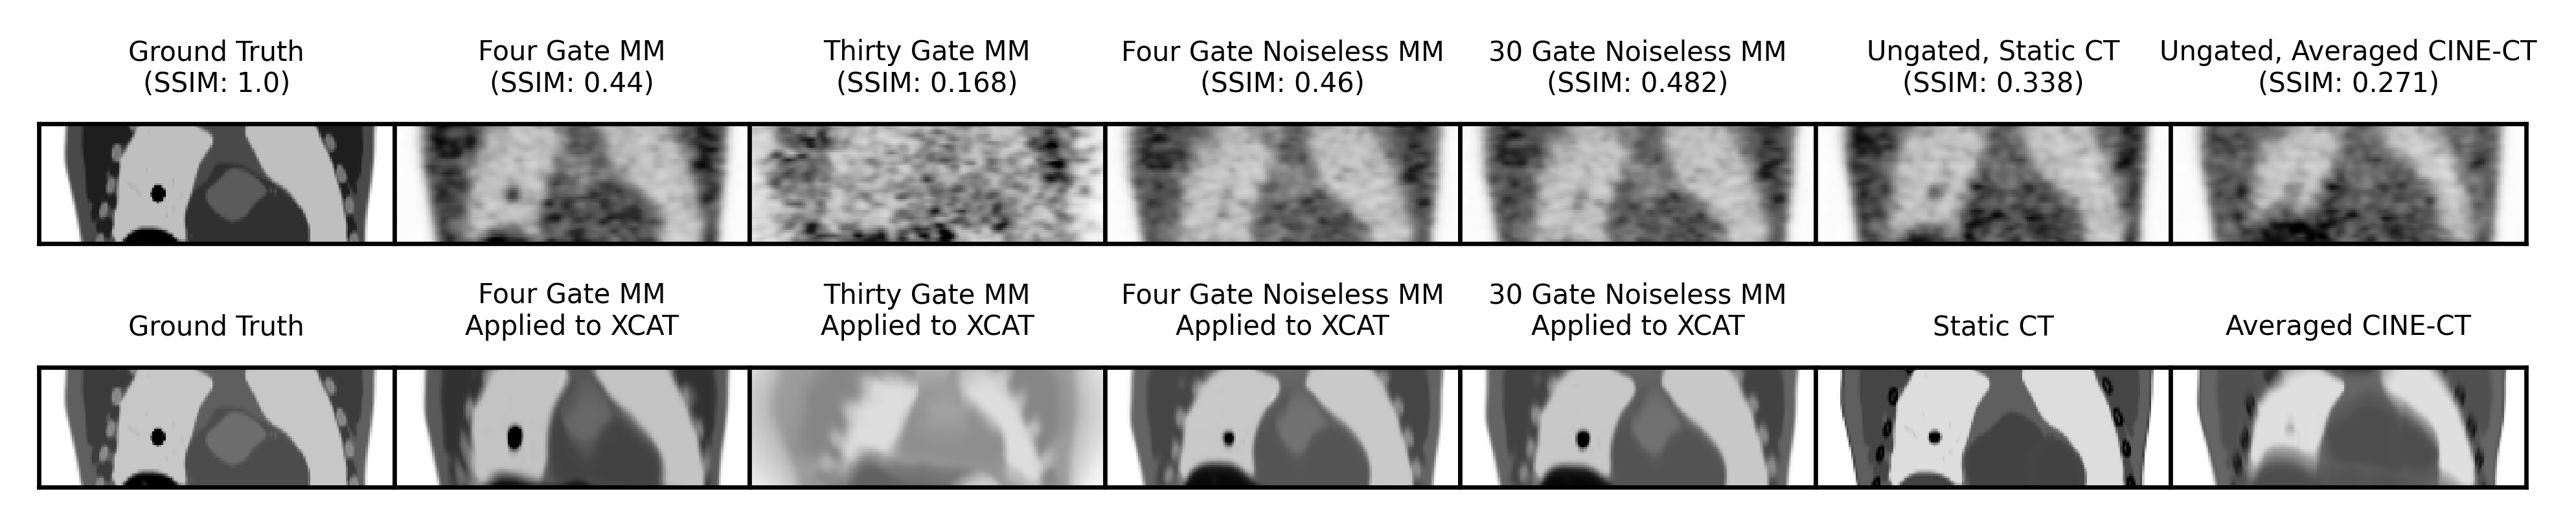
\includegraphics[width=1.0\linewidth]{visual_analysis.png}
        
        \begin{highlightbox}[UCLlightblue]
            \captionsetup{singlelinecheck=false, justification=centering}
            \caption{First row \gls{AC} \gls{MC} reconstructions, second row noiseless data. Colour map ranges consistent for all images in each column.}
        \end{highlightbox}
        
        \label{fig:visual_analysis}
    \end{figure}
\end{document}
